\documentclass[conference]{config/paper/IEEEtran}

\usepackage{config/paper/paper}
%--------------------------------------------------------------------%
%
% Hypenation untuk Bahasa Indonesia
%
% @author Petra Barus
%
%--------------------------------------------------------------------%
%
% Secara otomatis LaTeX dapat langsung memenggal kata dalam dokumen,
% tapi sering kali terdapat kesalahan dalam pemenggalan kata. Untuk
% memperbaiki kesalahan pemenggalan kata tertentu, cara pemenggalan
% kata tersebut dapat ditambahkan pada dokumen ini. Pemenggalan
% dilakukan dengan menambahkan karakter '-' pada suku kata yang
% perlu dipisahkan.
%
% Contoh pemenggalan kata 'analisa' dilakukan dengan 'a-na-li-sa'
%
%--------------------------------------------------------------------%

\hyphenation {
	% A
	%
	a-kan
	a-na-li-sa
	a-pli-ka-si
	% B
	%
	be-be-ra-pa
	ber-ge-rak
	% C
	%
	CAR-LA
	ca-ri
	% D
	%
	da-e-rah
	di-nya-ta-kan
	de-fi-ni-si
	% E
	%
	e-ner-gi
	eks-klu-sif
	% F
	%
	fa-si-li-tas
	% G
	%
	ga-bung-an
	% H
	%
	ha-lang-an
	% I
	% 
	i-nduk
	% J
	%
	% K
	%
	ka-me-ra
	kom-pu-ter
	kua-li-tas
	% L
	%
	% M
	%
	me-ngem-bang-kan
	% N
	%
	% O
	%
	% P
	%
	pe-ning-ka-tan
	% Q
	%
	% R
	%
	% S
	%
	se-de-mi-ki-an
	si-si
	% T
	% 
	tek-no-lo-gi
	% U
	%
	% V
	%
	% W
	%
	% X
	%
	% Y
	% 
	% Z
	%
}


% Adding references to the document
\addbibresource{IEEEabrv.bib}
\addbibresource{references.bib}

\IEEEoverridecommandlockouts
% The preceding line is only needed to identify funding in the first footnote. If that is unneeded, please comment it out.
\begin{document}

\title{Conference Paper Title*\\
{\footnotesize \textsuperscript{*}Note: Sub-titles are not captured in Xplore and
should not be used}
\thanks{Identify applicable funding agency here. If none, delete this.}
}

\author{\IEEEauthorblockN{1\textsuperscript{st} Given Name Surname}
	\IEEEauthorblockA{\textit{dept.\ name of organization (of Aff.)} \\
		\textit{name of organization (of Aff.)}\\
		City, Country \\
		email address or ORCID}
	\and
	\IEEEauthorblockN{2\textsuperscript{nd} Given Name Surname}
	\IEEEauthorblockA{\textit{dept.\ name of organization (of Aff.)} \\
		\textit{name of organization (of Aff.)}\\
		City, Country \\
		email address or ORCID}
	\and
	\IEEEauthorblockN{3\textsuperscript{rd} Given Name Surname}
	\IEEEauthorblockA{\textit{dept.\ name of organization (of Aff.)} \\
		\textit{name of organization (of Aff.)}\\
		City, Country \\
		email address or ORCID}
	\and
	\IEEEauthorblockN{4\textsuperscript{th} Given Name Surname}
	\IEEEauthorblockA{\textit{dept.\ name of organization (of Aff.)} \\
		\textit{name of organization (of Aff.)}\\
		City, Country \\
		email address or ORCID}
	\and
	\IEEEauthorblockN{5\textsuperscript{th} Given Name Surname}
	\IEEEauthorblockA{\textit{dept.\ name of organization (of Aff.)} \\
		\textit{name of organization (of Aff.)}\\
		City, Country \\
		email address or ORCID}
	\and
	\IEEEauthorblockN{6\textsuperscript{th} Given Name Surname}
	\IEEEauthorblockA{\textit{dept.\ name of organization (of Aff.)} \\
		\textit{name of organization (of Aff.)}\\
		City, Country \\
		email address or ORCID}
}

\maketitle

\begin{abstract}
	In the rising need for safe, inexpensive, easily accessible, and
	sustainable public transport in a densely-populated country like Indonesia,
	tram becomes a stand-out choice for its government. Along with the rise of
	autonomous vehicle technologies, trams can be made even safer by leveraging
	autonomous vehicle technology to make it operate autonomously.
	Unfortunately, in the development of autonomous trams, testing it on the
	real road would be expensive, dangerous, and time-consuming. Because of
	that, a simulation to test the software and hardware that is going to be
	used in the autonomous tram is needed.

	To do that, a communication mechanism to support the autonomous vehicle HILS
	system needs to be created. The research in this paper details the process
	of creating a communication mechanism for such systems. The communication
	mechanism is packaged in a library to increase its reusability and reduce
	its coupling with the simulation's main programs. The communication
	mechanism proposed by this paper boasts an average latency of only 10.99 ms
	which keeps the CARLA simulator running with 5--13 FPS. This communication
	mechanism also supports the use of CARLA virtual sensors so a simulation for
	autonomous vehicles can be done using the CARLA simulator.
\end{abstract}

\begin{IEEEkeywords}
	HILS communication, CARLA for HILS, autonomous vehicle simulation
\end{IEEEkeywords}

\section{Introduction}

A densely populated country, like Indonesia, needs public transportation that is
safe, inexpensive, easily accessible, and sustainable. One mode of public
transportation that can fulfill these four things is the electric tram. To
reduce potential accidents caused by human error, electric trams can take
advantage of artificial intelligence and control algorithms so that the trams do
not need a driver and can operate autonomously. This implies that trams can have
higher service times, reduce accidents, and increase safety
\cite{trilaksono_laporanRispro}.

The challenge in the development of artificial intelligence technology and
autonomous control algorithms is the need for a large number of tests.
Unfortunately doing the tests for the algorithm is expensive and time-consuming
when done in the real environment. Furthermore, it could be dangerous if the
algorithm is immature. Therefore, to reduce cost and time consumed doing tests,
the tests are done using simulations.

The simulation is run on a system with a hardware-in-the-loop (HILS) scheme. The
HILS system requires two computers to run properly: a computer to run the
simulator program and generate virtual sensor data (the CARLA simulator) as well
as a program to run simulation scenarios (called ``ScenarioRunner''); a computer
to be used on the tram which contains a program the control algorithm and
generates controls for the vehicle (called ``GRS''). The computer that runs
CARLA and ScenarioRunner is called SILS, while the computer that runs the GRS
program is called AGX/RKB.

Both ScenarioRunner and GRS need to communicate with each other to exchange
sensor data and tram control. The communication mechanism must not be too slow
so that it doesn't limit the simulation system's performance. AGX/RKB and SILS
computers are connected in a local area network (LAN) which implies an almost
ideal environment as the latency and interference in the network would be
minimum. Other than the performance issue, it is also important that the GRS
program can use the sensor data generated by CARLA and for ScenarioRunner to
consume tram control by GRS.

Currently, a HILS system for the project already exists. Unfortunately, in the
current implementation, the HILS system has bad performance and it also doesn't
support the use of virtual sensor data \cite{trilaksono_laporanRispro}. This
limits the usage of the simulation system so testing is still mostly done in the
real environment. This paper introduces a new approach for the HILS system which
uses a library that connects both programs while keeping the impact to the
system's performance to a minimum. The library is also able to transform virtual
sensor data from CARLA so it is usable by GRS.  With this library, both issues
existing in the current HILS system are remedied.
% The library also provides abstraction in the data parsing and exchange process
% in order to provide the best developer experience for the user of the library.
\section{Ease of Use}

\subsection{Maintaining the Integrity of the Specifications}

The IEEEtran class file is used to format your paper and style the text. All margins,
column widths, line spaces, and text fonts are prescribed; please do not
alter them. You may note peculiarities. For example, the head margin
measures proportionately more than is customary. This measurement
and others are deliberate, using specifications that anticipate your paper
as one part of the entire proceedings, and not as an independent document.
Please do not revise any of the current designations.
\section{System Overview}

In this research, a library called ``hils-connector'' is created. The purpose of
this library is to connect the ScenarioRunner and GRS program. The
``hils-connector'' is the interface that allows both programs to exchange data.
The library itself has two components: ``consumer'' (consumes sensor data, used
by GRS) and ``producer'' (produces sensor data by forwarding sensor data from
CARLA to consumer, used by ScenarioRunner).

The approach to use a library is chosen to reduce coupling between the library
and both main programs. The library can be loaded and linked optionally during
runtime and compile time to make better use of both computers' resources.

The communication protocol/method that is chosen for is ZeroMQ. ZeroMQ is chosen
because of its minimalism which could lead to improvement in communication
latency. Previously, ROS 2 was also considered, but ROS 2 has too many
abstraction layers and isn't supported by the OS version in AGX/RKB computer.
The AGX/RKB computer runs Ubuntu 18.04 which only supports up to ROS 1. Although
a bridge between ROS 2 and ROS 1, that bridge would only add overhead in the
communication process, therefore ROS was not chosen. Another communication
protocol that was considered is HTTP, which is used in the previous HILS system.
HTTP is also not chosen because of the additional overhead needed to parse
header and status code which is not needed in the HILS system. Thus, to maximize
the usage of computer resource and reduce possible overhead, ZeroMQ is chosen
over HTTP.

With this library approach, the system architecture can be seen in
Fig.~\ref{section-3-hils-deployment-diagram}. The two main programs,
ScenarioRunner and GRS, are connected to each other using hils-connector in a
local area network. Each library components are then connected using ZeroMQ.
CARLA is connected to the ScenarioRunner program using the CARLA Python API
through function calls.

\begin{figure}[htbp]
	\centerline{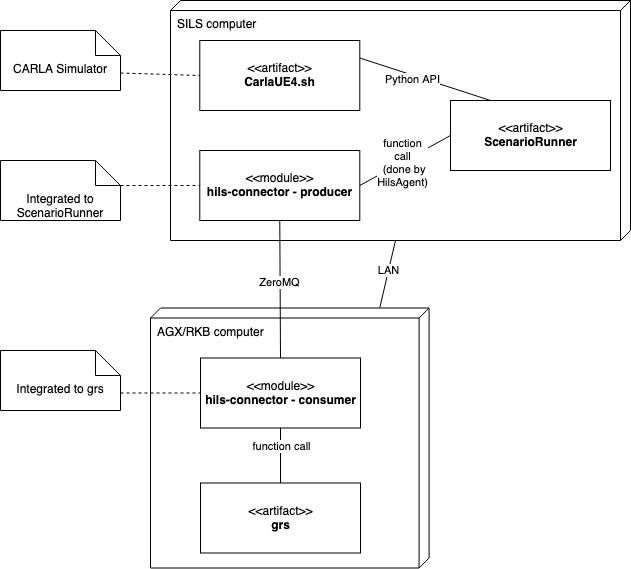
\includegraphics[width=0.4\textwidth]{resources/chapter-3/deployment-diagram-new-hils-EN.png}}
	\caption{HILS System Architecture}
	\label{section-3-hils-deployment-diagram}
\end{figure}

Then, as for how the system runs, it can be seen in
Fig.~\ref{section-3-hils-sequence-diagram}. Do note ScenarioRunner is called
``HILS agent'' in the diagram because HILS agent is the agent that is ran on
ScenarioRunner. To summarize how the system works:
\begin{enumerate}
	\item when CARLA steps, a sensor data is emitted,
	\item the producer component pushes it to the ZeroMQ socket,
	\item the consumer component waits for sensor data then pull from each
	      ZeroMQ socket,
	\item GRS will process that data to generate a control,
	\item the consumer component pushes the control to the ZeroMQ socket,
	\item the producer component will pull it and then send it to the
	      ScenarioRunner program, and
	\item ScenarioRunner will then apply the control to CARLA.
\end{enumerate}

\begin{figure}[htbp]
	\centerline{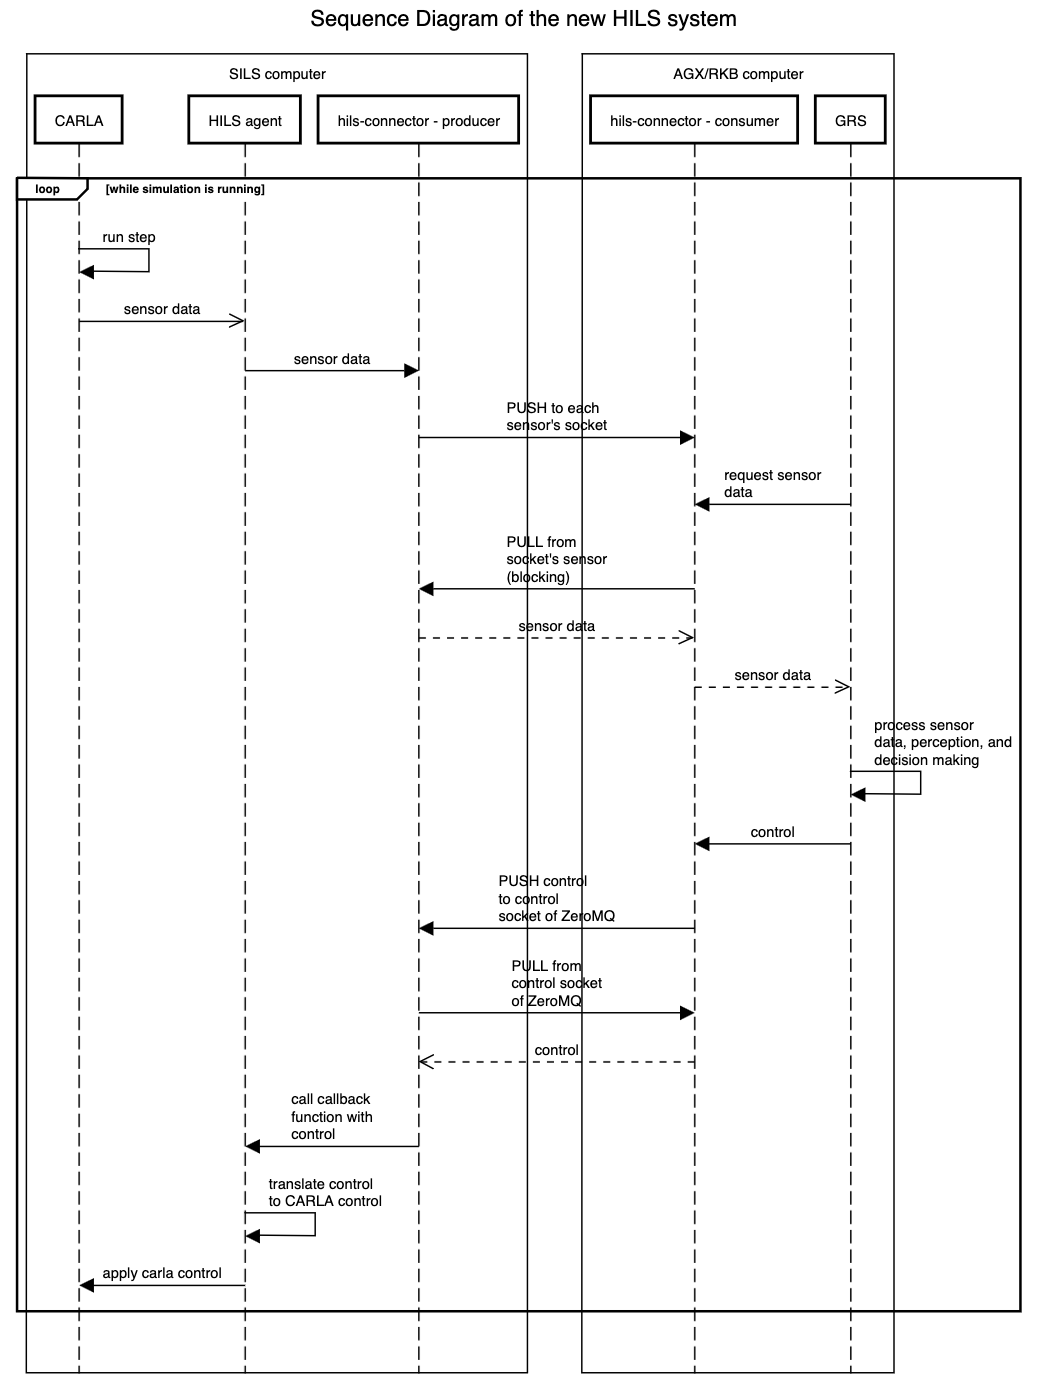
\includegraphics[width=0.5\textwidth]{resources/chapter-3/sequence-diagram-new-hils-kasar-EN.png}}
	\caption{HILS System Architecture}
	\label{section-3-hils-sequence-diagram}
\end{figure}

% \begin{table}[htbp]
% 	\caption{Table Type Styles}
% 	\label{tab1}
% 	\begin{center}
% 		\begin{tabular}{c c c c}
% 			\toprule
% 			\textbf{Table} & \multicolumn{3}{|c|}{\textbf{Table Column Head}}                                                         \\
% 			\cline{2-4}
% 			\textbf{Head}  & \textbf{\textit{Table column subhead}}           & \textbf{\textit{Subhead}} & \textbf{\textit{Subhead}} \\
% 			\midrule
% 			copy           & More table copy$^{\mathrm{a}}$                   &                           &                           \\
% 			\bottomrule
% 			\multicolumn{4}{l}{$^{\mathrm{a}}$Sample of a Table footnote.}
% 		\end{tabular}
% 	\end{center}
% \end{table}


\section*{Acknowledgment}

The preferred spelling of the word ``acknowledgment'' in America is without
an ``e'' after the ``g''. Avoid the stilted expression ``one of us (R. B.
G.) thanks $\ldots$''. Instead, try ``R. B. G. thanks$\ldots$''. Put sponsor

\printbibliography

\vspace{12pt}
\color{red}
IEEE conference templates contain guidance text for composing and formatting conference papers. Please ensure that all template text is removed from your conference paper prior to submission to the conference. Failure to remove the template text from your paper may result in your paper not being published.

\end{document}